% Context

Rocky, icy, and metallic objects in space, smaller than asteroids, are called cosmic dust. Cosmic dust is created as debris of collisions of larger objects, but also by condensation of gases, or by being expelled from a~larger body, such as a~comet or a~moon with active volcanism. Cosmic dust which originates in the~solar system is called interplanetary dust, as opposed to cosmic dust which occupies the~interstellar or intergalactic space. The~circumsolar interplanetary dust is responsible for zodiacal light, which is the~diffuse glow observed in post-sunset and pre-sunrise night sky near the~ecliptic plane, shown in Fig.~\ref{fig:zodiacal_light}.

\begin{figure}[t]
 	\centering
 	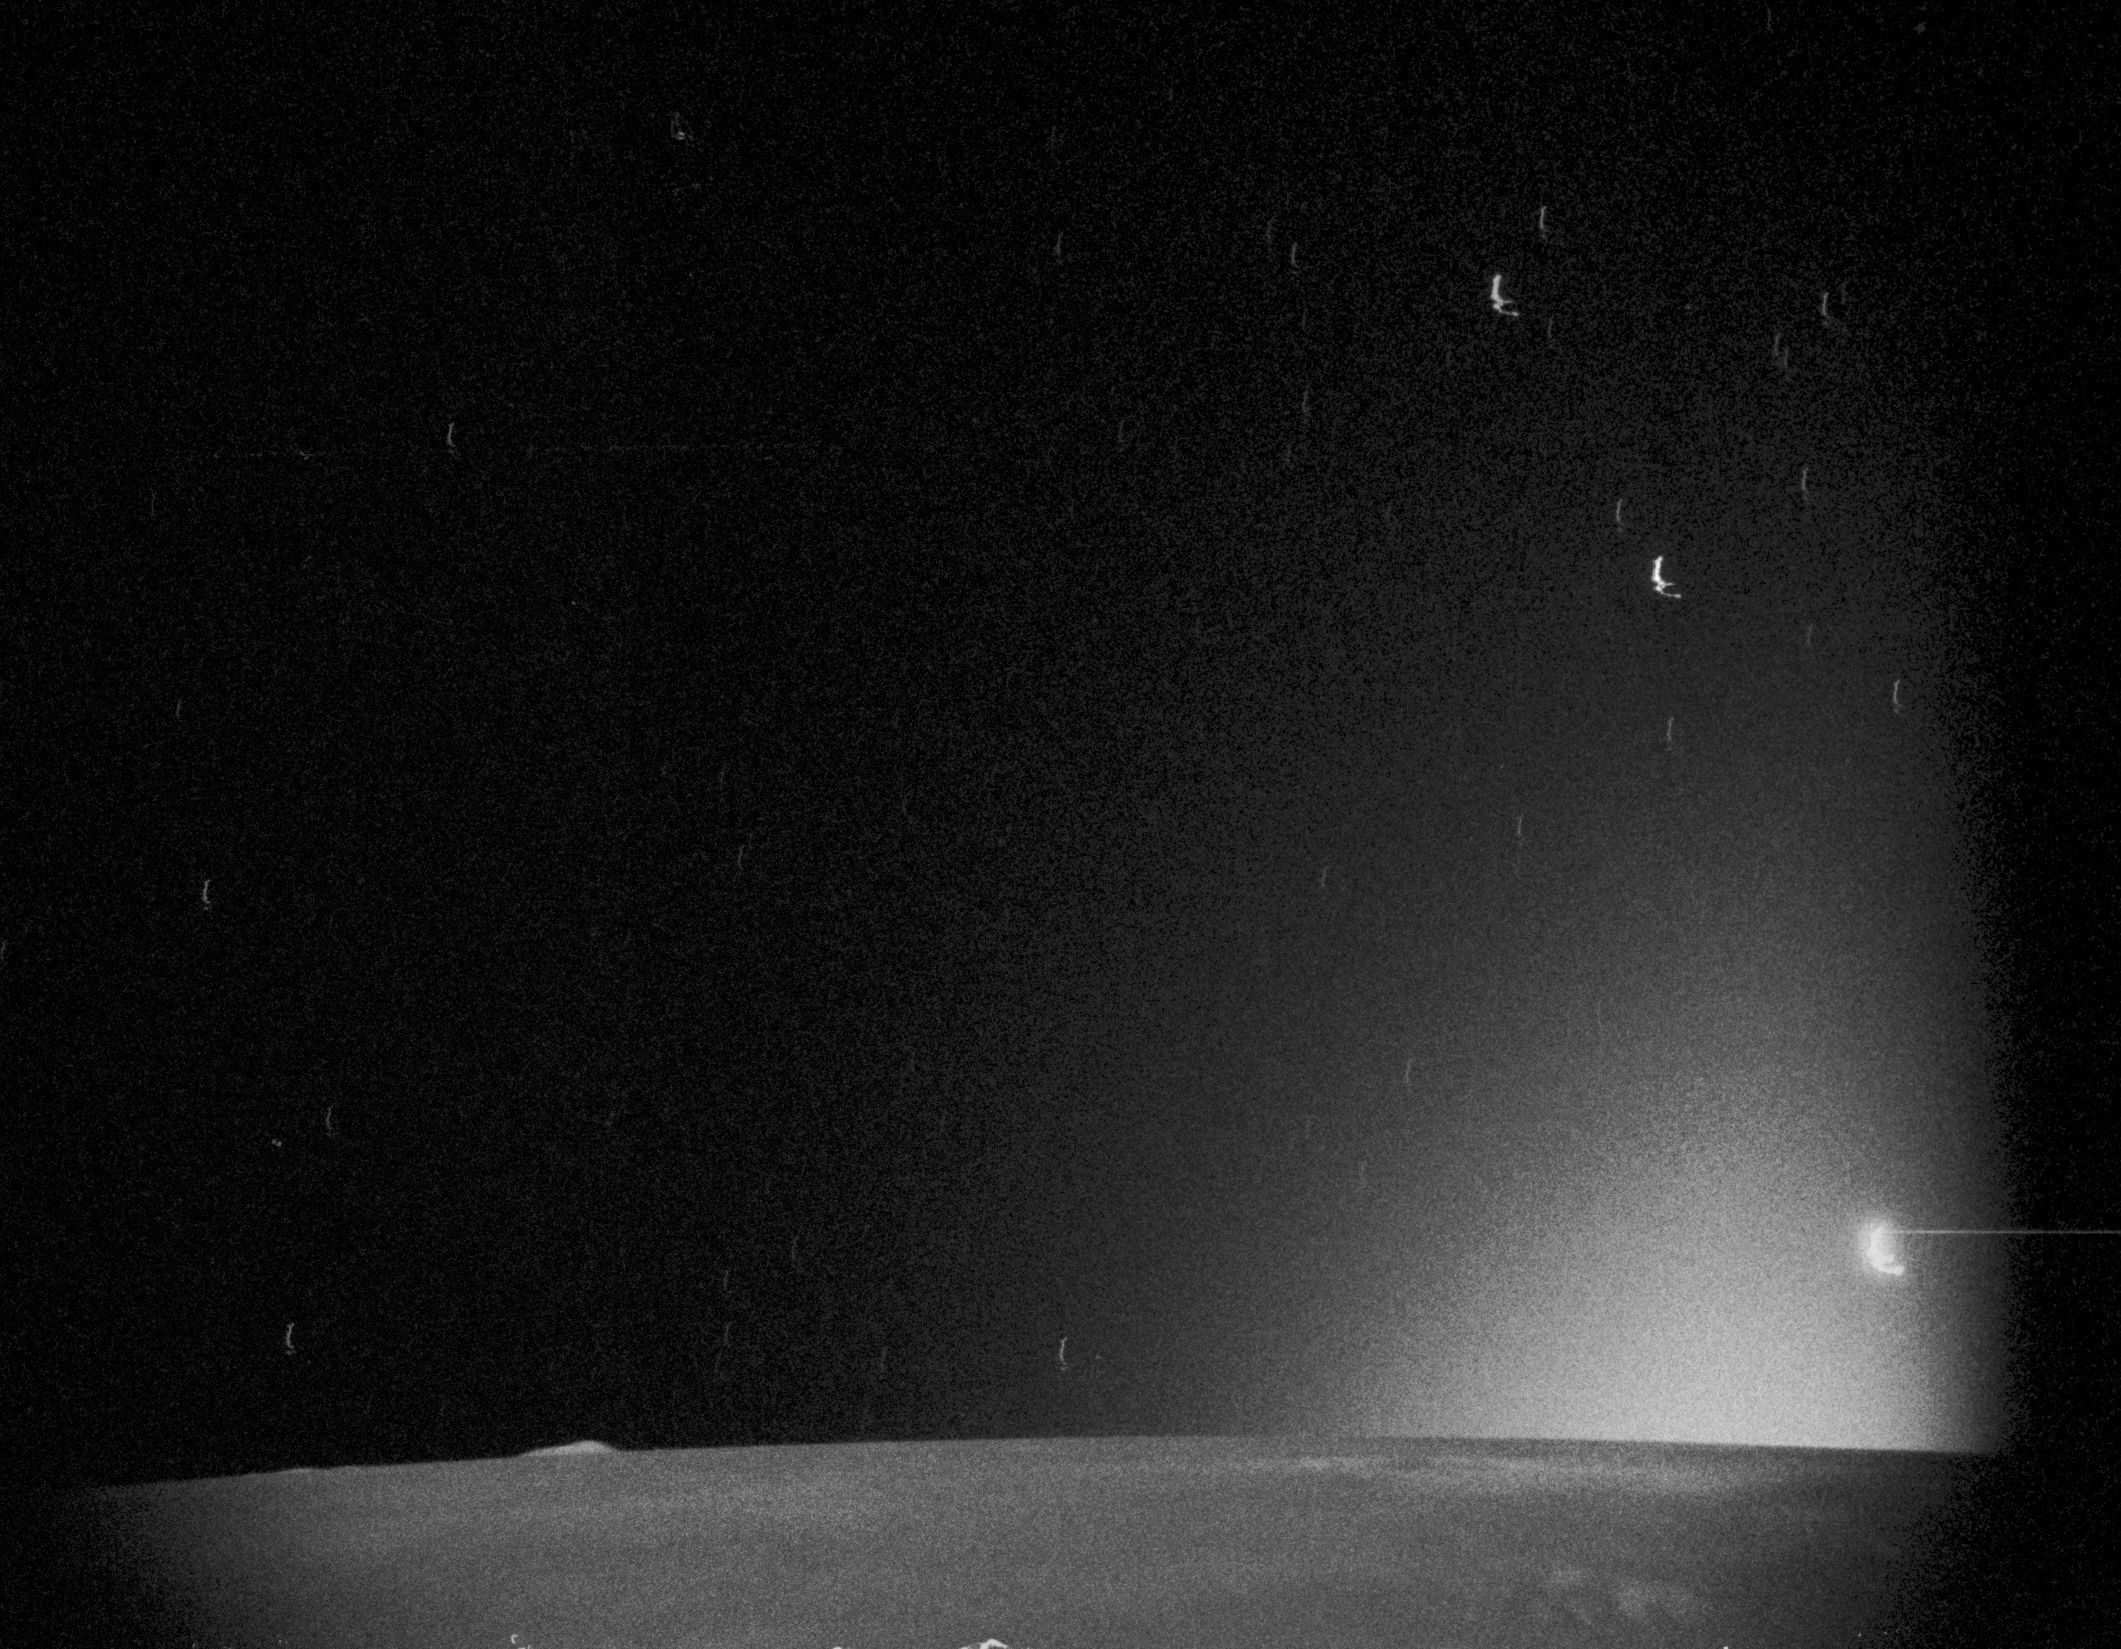
\includegraphics[width=8cm]{figures/zodiacal_light.jpg}
 	\caption{A long-exposure photo from the~orbit of the~Moon, taken shortly after sunset on July 31\textsuperscript{st}, 1971. By NASA - Magazine 98, Apollo 15, March to the~Moon.}
 	\label{fig:zodiacal_light}
\end{figure}

The~interplanetary dust cloud is an integral part of the~solar system, and its dynamics contains information about the~past and the~present of other bodies. In the~inner solar system, micron-sized dust is a~probe into the~vicinity of the~Sun. When it gets too close to the~Sun, it is destroyed by the~extreme near-solar conditions, which forms a~dust-free zone around the~Sun. By understanding how the~circumsolar dust moves, where the~collisions happen, where it is destroyed, and how its characteristics depend on its composition, we find more about the~conditions around the~Sun, which influence the~rest of the~solar system. For example, when a~dust grain is sputtered or evaporated by the~Sun, its material enters the~solar wind and is carried out of the~inner solar system. With understanding of the~dust dynamics in the~solar system, the~study of other stars' circumstellar dust clouds and planetary disks is also enabled.

The~atmosphere of the~Earth offers a~great target for cosmic dust, and the~cosmic dust of more than $\SI{100}{\mu m}$ entering the~atmosphere is observable in the~form of meteors. The~vapors ablated from dust influence the~mesosphere and the~troposphere. Most meteors are of interplanetary origin. The~amount of dust entering the~atmosphere was estimated decades ago and remains fairly uncertain. One of the~reasons for this is the~vast range of the~mass of grains which contribute to the~influx.

When spacecraft move through a~dusty environment, such as the~inner solar system, they randomly collide with dust grains of the~dust cloud. Most of the~collisions in the~inner solar system are with sub-micron sized dust. Little can be told about the~dust cloud based on a~single collision, but based on many collisions, generalizations can be made about the~size and speed distribution within the~cloud. 

This thesis is mostly concerned with measurements done by two spacecraft: Solar Orbiter (SolO) and Parker Solar Probe (PSP). Both are Sun-orbiting spacecraft, and are the~two human made objects which venture the~closest to the~Sun. Using their electrical antennas to register collisions with dust grains, they provide dust measurements from the~region where no other spacecraft have measured before. This alone makes their measurements valuable, and the~fact that they operate simultaneously and over several years only more so.

To understand the~dynamics in the~interplanetary dust cloud, we make use of the~similarities and differences between the~two spacecraft. Different statistical modeling approaches must be taken to yield the~maximum information in different regions. In the~region further away from the~Sun, collisions with dust grains are rare. Here, reliable and consistent detection in combination with counting statistics reveals the~spatial distribution. In the~close vicinity of the~Sun, several processes occur at the~same time. Here, we identify the~most important dust properties by comparing measurements to models. By applying the~appropriate tools, we extend the~current understanding of the~dust grains' speed, masses, collisions, and location in different regions in the~inner solar system.

% Outline

The~aim of this thesis is to extend the~understanding of the~interplanetary dust inside Earth's orbit from electrical antenna measurements performed by two unique spacecraft, SolO and PSP. We achieve this by taking a~more mathematically precise approach than what was used previously. Single-grain dust properties, as well as forces acting on individual dust grains are introduced in Ch. \ref{ch:forces}. Dust grains in the~Solar system compose the~interplanetary dust cloud, in which grains of similar properties follow similar trajectories. These form individual dust populations, which are introduced in Ch. \ref{ch:populations}. To yield the~most information possible, sharp statistical tools are needed, some of which are introduced in Ch. \ref{ch:statistics}. The~dust detection principles are described in Ch. \ref{ch:detection}, where emphasis is put on antenna measurements. The~articles, which make up a~part of this thesis, are described in Ch. \ref{ch:sum-paper}. Finally, Ch. \ref{ch:conclusion} concludes and offers an outlook.